\chapter{Implementation}
\label{chapter:Implementation}

This chapter describes the main modules written by Python and Julia.
The structure of each neural network is also described.


\section{Summary of external modules for this experiments}

\subsection{AutomotiveDrivingModels.jl}

A Julia package containing tools for automotive simulations in 2D.

\subsection{NGSIM.jl}

A Julia package for working with the Next Generation Simulation dataset ({\tt NGSIM}). Was tested on the Highway 101 and I-80 datasets.

This package is fully compatible with {\tt AutomotiveDrivingModels.jl}, providing the {\it Roadway} and {\it Trajdata} types from the {\tt NGSIM} data. Roadway geometry was extracted from the {\tt NGSIM} CAD files. The vehicle trajectories were filtered to provide better global positions and orientation.

The {\tt NGSIM} trajectory data is available in our first release, with instructions here.

\subsection{AutoViz.jl}

A package for rendering simple scenes primarily consisting of cars on roadways using Cairo.

AutoViz is undergoing significant changes.

\begin{figure}[H]
\begin{center}
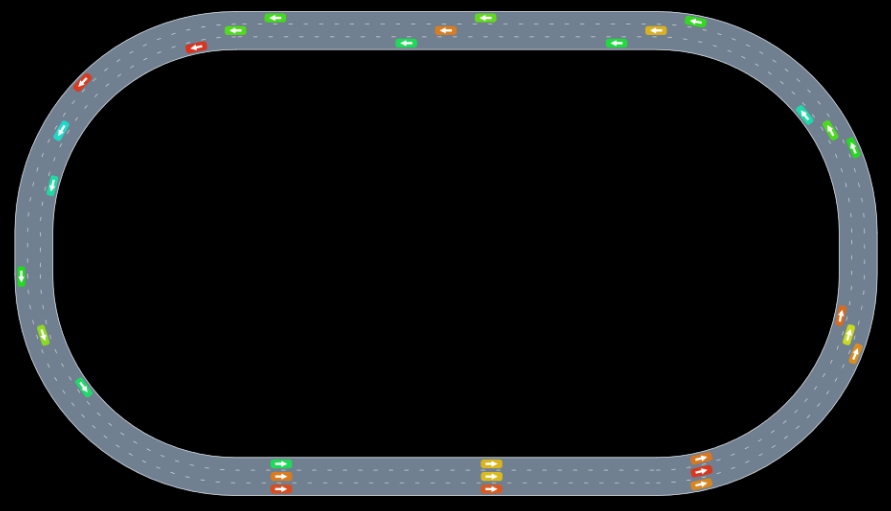
\includegraphics[width=10cm]{./figures/readmeimage.png}
\caption{AutoViz demo.}
\label{fig:example_autoviz_demo}
\end{center}
\end{figure}


\subsection{ForwardNets.jl}

A simple Julia package for neural networks.

\subsection{AutoDrivers.jl}

Advanced human driving models for {\tt AutomotiveDrivingModels.jl}.

\subsection{gail-driver}

Utilities and scripts used to perform experiments described in "Imitating Driver Behavior with Generative Adversarial Networks". Built on rllab and source code for generative adversarial imitation learning.


\subsection{rllab}

{\tt rllab} is a framework for developing and evaluating reinforcement learning algorithms. It includes a wide range of continuous control tasks plus implementations of the following algorithms:

\begin{itemize}
\item    REINFORCE
\item    Truncated Natural Policy Gradient
\item    Reward-Weighted Regression
\item    Relative Entropy Policy Search
\item    Trust Region Policy Optimization
\item    Cross Entropy Method
\item    Covariance Matrix Adaption Evolution Strategy
\item    Deep Deterministic Policy Gradient
\end{itemize}

{\tt rllab} is fully compatible with {\tt OpenAI Gym}. See here for instructions and examples.

{\tt rllab} comes with support for running reinforcement learning experiments on an EC2 cluster, and tools for visualizing the results. See the documentation for details.

The main modules use {\tt Theano} as the underlying framework, and we have support for {\tt TensorFlow} under {\tt sandbox/rocky/tf}.


\section{Software structure summary}

The program is roughly divided into a training program consisting of Python and Julia and a validation program consisting only of Julia.

The following diagrams will be inserted.
\begin{itemize}
\item class diagrams of important classes.
\item relation of data and modules
\end{itemize}




Now writing...


\subsection{Training program summary}

All vehicle behavior is described by the Julia program. The discriminator network is implemented in python's tensorflow.
policy network is a ForwardNets module by Julia, but uses python's tensorflow to configure the network.



\subsection{Validation program summary}

All vehicle behavior is described by the Julia program. 
Policy is also written in Julia.
The validation program does not update Policy. It also doesn't use the discriminator, so it doesn't use Python code.

Now writing...


\section{Features for observation}

This is all the data that the vehicle observes while driving. The data consists of the relative position of another vehicle seen from the own vehicle around the vehicle as a reflection of virtual LiDAR, odometry, and other indicators.

Observation includes 51 elements of scalars.

\begin{itemize}
\item 20 directions of Lidar beam range $[m]$
\item 20 directions of Lidar beam range rate $[m/s]$

\begin{figure}[H]
\begin{center}
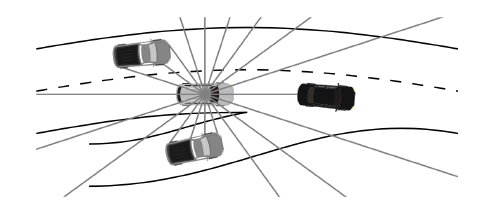
\includegraphics[width=10cm]{./figures/lidar_beam.png}
\caption{20 lidar beams(range and range-rate)}
\label{fig:lidar_beam}
\end{center}
\end{figure}

Range is the distance to another vehicle observed in the LiDAR beam direction.
The range rate is the velocity (in the beam direction) of another vehicle observed in the LiDAR beam direction.

\item speed of ego vehicle. $[m/s]$

Speed is a scalar value, longitudinal speed to the lane direction.

\item vehicle length $[m]$

Bounding box size of vehicle heading direction.

\item vehicle width $[m]$

Bounding box size of vehicle perpendicular heading direction.

\item lane offset $[m]$

Lateral distance from lane center.

\item lane relative heading $[rad]$
\item lane curvature $[m^{-1}]$
\item marker distance (L) $[m]$

Distance to the left edge of the road.

\item marker distance (R) $[m]$

Distance to the right edge of the road.

\item 3 indicators in ${0, 1}$ value for undesirable  states.
\end{itemize}

3 indicators are used to identify when the ego vehicle encountered undesirable states, such as collision, off-road and reverse.
If there are undesirable states, the correspondent  indicator shows 1 otherwise 0.





\subsection{Input/output of policies}

Policy's inputs are 51 elements as observation.

Policies outputs are 2 elements as action.
Action is as follows.

\begin{itemize}
\item acceleration $[m/s^2]$
\item turn rate $[rad/s]$
\end{itemize}


\subsection{Input/output for discriminator}

Discriminator's input is a 51 element vector as an observation and an action. (total 53 elements)

Discriminator's output is a bit. "1" means it is an expert policy.



\section{Metrics}


This section details the metrics for vehicle behavior that are evaluated by the validation program.

Speed, acceleration and jerk are calculated from the sample point to be calculated and the sample point one previous point (0.1 second before).
Speed is calculated from the position of the sample point and the position of the previous sample point, acceleration is calculated from the speed of the sample point and the speed of previous sample point, jerk is calculated from the acceleration of the sample point and the acceleration of the previous sample point.
Future sample points are not used.

\begin{comment}
速度、加速度、jerk は、計算を行うサンプル点とそのひとつ前(0.1秒前のサンプル点)から計算する。
速度は、サンプル点と一つ前のサンプル点の位置から計算され、加速度は、サンプル点と一つ前のサンプル点の速度から計算され、jerkは、サンプル点と一つ前のサンプル点の加速度から計算される。
未来のサンプル点は使用されていない。

サンプルは1秒に10回(つまり10Hz)行われ、トラジェクトリは10秒間である。一つのトラジェクトリは100のサンプルポイントからなる。
\end{comment}

The sample is taken 10 times per second (ie 10Hz) and the trajectory is 10 seconds. Therefore, one trajectory consists of 100 sample points.
The following metrics are calculated on that basis.

\begin{itemize}
\item Root Weighted Square Error.

The square of the two-dimensional distance, lateral distance, and speed difference between the expert vehicle and the learning vehicle. The smaller value means learning policy is more similar to the expert.

\begin{itemize}
\item Position

2 dimensional distance. 
 
\item Lane Offset

Lateral distance from lane center.

\item Speed

Longitudinal speed of vehicle heading direction.

\end{itemize}
\item Kullback-Leibler Divergence.

The KL divergence of the probability distributions of the expert policy $\pi_E$ and the reinforcement learning policy $\pi_\theta$ is shown. The smaller  value means the learning policy is more similar to the expert.

\begin{itemize}
\item iTTC

Inverse time to collision.

\item Speed

Longitudinal speed of vehicle heading direction.

\item Acceleration

Longitudinal acceleration of vehicle heading direction.

\item Turn-Rate

Turn-rate of vehicle heading.

\item Jerk

Longitudinal jerk of vehicle heading direction.

\end{itemize}




\item Emergent Value.

It is a metric for unfavorable driving, such as emergency braking or running off the track. The smaller values means driving is safety.
In the following metrics, 1 represents once.
There are 100 sample points on the trajectory, 
offroad-rate is 100.0 if all the trajectories are off the track.
Only collision is calculated so that the maximum value of one trajectory is 1.

All the calculation methods follow the original paper.\cite{DBLP:journals/corr/KueflerMWK17}


\begin{itemize}

\item Lane Change Rate

It is the number of lane changes made in 10 seconds.

\item Offroad Duration

It is the number of spent off road in 10 seconds.

\item Collision Rate

It is the number of collision made in 10 seconds.

\item Hard Break Rate

It is the number of spent hard break in 10 seconds.

\end{itemize}
\end{itemize}


\section{Reward network summary}

Reward network is a discriminator and is realized by tensorflow. The surrogate reward is calculated based on the discrimination result by this network.

\begin{table}[H]
\centering
\begin{tabular}{|c|r|r|}
\hline 
layer  & weight   & bias \\ \hline \hline
input  & 53 $\times$ 256 & 256  \\
hidden & 256 $\times$ 128 & 128 \\ 
hidden & 128 $\times$ 64 & 64 \\ 
hidden & 64 $\times$ 64 & 64 \\ 
hidden & 64 $\times$ 32 & 32 \\ 
output & 32 $\times$ 1 & 1 \\ 
\hline
\end{tabular} 
\caption{}
\label{tab:reward_network}
\end{table}


\begin{itemize}
\item location in sourcecode.
\item specification
\end{itemize}


\section{Policy network summary}

\begin{comment}
本実験では、ポリシタイプはMLPとGRUの二通りの実験を行っている。MLPは通常の多層パーセプトロンであり、フィードフォワードの接続だけで作られている。GRUはリカレント層を持ち、現在の状態は過去の状態の影響を受ける。ここに、実験でポリシとして使用されたニューラルネットワークの構造を示す。
\end{comment}

In this experiment, two types of experiments, {\it MLP} and {\it GRU}, are performed. The {\it MLP} is a regular multi-layer perceptron, made entirely of feedforward connections. {\it GRU} has a recurrent layer, and its current state is affected by past states. Here is the structure of the neural network used as a policy in the experiment.





\subsection{GRU structure}


\begin{table}[H]
\centering
\begin{tabular}{|c|r|}
\hline 
layer  & weight    \\ \hline \hline
w\_hc  & 32 $\times$ 32   \\
w\_hr  & 32 $\times$ 32   \\
w\_hu  & 32 $\times$ 32   \\
w\_xc  & 32 $\times$ 32   \\
w\_xr  & 32 $\times$ 32   \\
w\_xu  & 32 $\times$ 32   \\
b\_c  & 32   \\
b\_r  & 32   \\
b\_u  & 32   \\
output & 32 $\times$ 2   \\
output bias & 2   \\
\hline
\end{tabular} 
\caption{GRU network gru layer}
\label{tab:reward_gru_gru_network}
\end{table}

\begin{table}[H]
\centering
\begin{tabular}{|c|r|r|}
\hline 
layer  & weight   & bias \\ \hline \hline
input  & 51 $\times$ 256 & 256  \\
hidden0 & 256 $\times$ 128 & 128 \\
hidden1 & 128 $\times$ 64  & 64  \\
hidden2 & 64 $\times$ 64   & 64  \\
hidden3 & 64 $\times$ 32   & 32  \\
hidden4 & 32 $\times$ 32   & 32  \\
output & 32 $\times$ 2    & 2  \\
\hline
\end{tabular} 
\caption{GRU network mlp layer}
\label{tab:reward_gru_mlp_network}
\end{table}


\begin{itemize}
\item location in sourcecode.
\item specification
\end{itemize}

\subsection{MLP structure}



\begin{table}[H]
\centering
\begin{tabular}{|c|r|r|}
\hline 
layer  & weight   & bias \\ \hline \hline
input  & 51 $\times$ 256 & 256  \\
hidden0 & 256 $\times$ 128 & 128 \\
hidden1 & 128 $\times$ 64  & 64  \\
hidden2 & 64 $\times$ 64   & 64  \\
output & 64 $\times$ 32   & 32  \\
\hline
\end{tabular} 
\caption{MLP network layer}
\label{tab:reward_mlp_network}
\end{table}



\begin{itemize}
\item location in sourcecode.
\item specification
\end{itemize}

\pagebreak
\section{Summary of environment}

To support the development of algorithms for driver behavior at microscopic levels, the Next Generation SIMulation ({\it NGSIM}) computer program is collecting detailed, high-quality traffic datasets. {\it NGSIM} stakeholder groups identified the collection of real-world vehicle trajectory data as important to understanding and researching driver behavior at microscopic levels. The {\it NGSIM} datasets represent the most detailed and accurate field data collected to date for traffic microsimulation research and development. 





Dataset for this experiment is as follows.


\subsection{Interstate 80 Freeway Dataset(Publication Number: FHWA-HRT-06-137)}

The Interstate 80 (I-80) freeway dataset was the first of several datasets collected under the {\it NGSIM} program.

Researchers for the {\it NGSIM} program collected detailed vehicle trajectory data on eastbound I-80 in the San Francisco Bay area in Emeryville, CA, on April 13, 2005. The study area was approximately 500 meters (1,640 feet) in length and consisted of six freeway lanes, including a high-occupancy vehicle (HOV) lane. An onramp also was located within the study area. Seven synchronized digital video cameras, mounted from the top of a 30-story building adjacent to the freeway, recorded vehicles passing through the study area. NG-VIDEO, a customized software application developed for the {\it NGSIM} program, transcribed the vehicle trajectory data from the video. This vehicle trajectory data provided the precise location of each vehicle within the study area every one-tenth of a second, resulting in detailed lane positions and locations relative to other vehicles. 

A total of 45 minutes of data are available in the full dataset, segmented into three 15-minute periods: 4:00 p.m. to 4:15 p.m.; 5:00 p.m. to 5:15 p.m.; and 5:15 p.m. to 5:30 p.m. These periods represent the buildup of congestion, or the transition between uncongested and congested conditions, and full congestion during the peak period. In addition to the vehicle trajectory data, the I-80 dataset also contains computer-aided design and geographic information system files, aerial orthorectified photos, freeway loop detector data within and surrounding the study area, raw and processed video, signal timing settings on adjacent arterial roads, traffic sign information and locations, weather data, and aggregate data analysis reports.

The full I-80 dataset is freely available at the {\it NGSIM} Web site at \url{http://ops.fhwa.dot.gov/trafficanalysistools/ngsim.htm}.

\begin{figure}[H]
\begin{center}
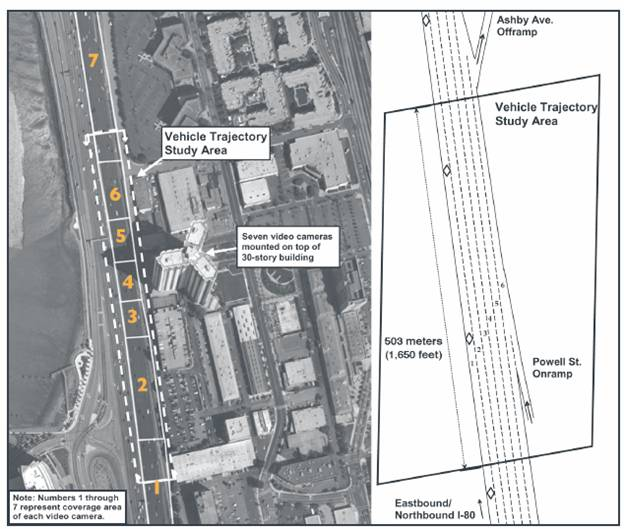
\includegraphics[width=7cm]{./figures/image137b.jpg}
\caption{Interstate 80 Freeway}
\label{fig:pict_us80}
\end{center}
\end{figure}


\subsection{US Highway 101 Dataset(Publication Number: FHWA-HRT-07-030)}

The US Highway 101 (US 101) dataset was one of several datasets collected under the NGSIM program.
Description

Researchers for the {\it NGSIM} program collected detailed vehicle trajectory data on southbound US 101, also known as the Hollywood Freeway, in Los Angeles, CA, on June 15th, 2005. The study area was approximately 640 meters (2,100 feet) in length and consisted of five mainline lanes throughout the section. An auxiliary lane is present through a portion of the corridor between the on-ramp at Ventura Boulevard and the off-ramp at Cahuenga Boulevard. Eight synchronized digital video cameras, mounted from the top of a 36-story building adjacent to the freeway, recorded vehicles passing through the study area. NG-VIDEO, a customized software application developed for the {\it NGSIM} program, transcribed the vehicle trajectory data from the video. This vehicle trajectory data provided the precise location of each vehicle within the study area every one-tenth of a second, resulting in detailed lane positions and locations relative to other vehicles.

A total of 45 minutes of data are available in the full dataset, segmented into three 15 minute periods: 7:50 a.m. to 8:05 a.m.; 8:05 a.m. to 8:20 a.m.; and 8:20 a.m. to 8:35 a.m.

These periods represent the buildup of congestion, or the transition between uncongested and congested conditions, and full congestion during the peak period. In addition to the vehicle trajectory data, the US 101 dataset also contains computer-aided design and geographic information system files, aerial ortho-rectified photos, loop detector data, raw and processed video, weather data, and aggregate data analysis reports.

The full US 101 dataset is freely available at the {\it NGSIM} Web site at \url{http://ops.fhwa.dot.gov/trafficanalysistools/ngsim.htm}.

Travelers in freeway merge areas face complex tasks in executing their short term trip plans. They must accelerate to the predominant through speeds, check for acceptable gaps, and position themselves for their next maneuvers. During medium and heavy congestion, these tasks are complicated by the volume of other travelers competing for space on crowded freeways.

In reality, travelers often overcome some of this complexity by cooperating with other drivers. Existing microsimulation models generally use basic or modified versions of lane changing models to model freeway merging behaviors. While these models do account for gaps created by adjacent vehicles, and in some cases model reduced gap acceptance thresholds during congested conditions, the models do not explicitly account for cooperation among drivers. As a result, existing models tend to overpredict congestion because the models fail to capture localized system optimization that occurs when drivers exhibit cooperative behaviors.

{\it NGSIM} researchers used the US 101 dataset to develop and validate a new driver behavior model, the Cooperative/Forced Freeway Merge model, which models lane changing on a freeway merge and weaving section that treats driver cooperation explicitly.

\begin{figure}[H]
\begin{center}
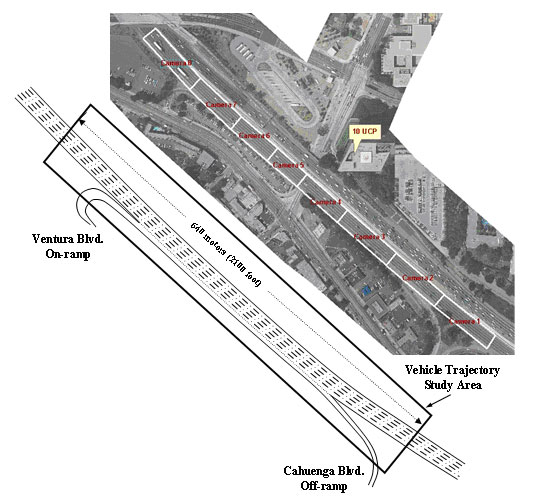
\includegraphics[width=7cm]{./figures/07030fig1.jpg}
\caption{US highway 101}
\label{fig:pict_us101}
\end{center}
\end{figure}







\section{Changes to the original program}


List of the original program and the changes will be inserted.


\subsection{Julia version problem}

Original program is based on Julia 0.5. 
Since JULIA that can be used in this experiment is limited to version 0.6 or later, grammatical corrections were made.

\subsubsection{AbstructType definition}

Old style definition is as follows.

\begin{lstlisting}[caption=Julia old style definition ,label=list:julia_05_def, escapechar=!, language=Pascal, frame=single]
abstract UserType                          # definition of abstract type
a = Array(ArrayElement, size)              # definition of array
\end{lstlisting}



\begin{lstlisting}[caption=Julia 0.6 style ,label=list:julia_06_def, escapechar=!, language=Pascal, frame=single]
abstract type UserType end                 # definition of abstract type
a = Array{ArrayElement}(size)              # definition of array
\end{lstlisting}


\subsubsection{ForwardNets.jl/variable.jl}

Old style definition is as follows.

\begin{lstlisting}[caption=Julia old style definition 
,label=list:julia_05_forwardnets, language=Pascal, frame=single]
function Base.push!{T}(net::ForwardNet{T}, ::Type{Variable},
    name::Symbol,
    shape::Int...
    )

    push!(net, Variable(name, Array(T, shape...)))
end
function Base.push!{T}(net::ForwardNet{T}, ::Type{Variable},
    name::Symbol,
    parent::NameOrIndex,
    )

    node = Variable(name, output(net[parent]))
    push!(net, node, parent)
end
\end{lstlisting}

Each push function is defined twice, but it is an error because the argument is ambiguous. Avoiding the ambiguity by giving an extra dummy argument to the second function.
Changed code is as follows.

\begin{lstlisting}[caption=Changed code 
,label=list:julia_06_forwardnets, language=Pascal, frame=single]
function Base.push!{T}(net::ForwardNet{T}, ::Type{Variable},
    name::Symbol,
    shape::Int...
    )

    push!(net, Variable(name, Array{T}(shape...)))
end
function Base.push!{T}(net::ForwardNet{T}, ::Type{Variable},
    name::Symbol,
    parent::NameOrIndex,
    ::Symbol      # dummy symbol inserted
    )

    node = Variable(name, output(net[parent]))
    push!(net, node, parent)
end
\end{lstlisting}

\subsubsection{AutomotiveDrivingModels.jl/src/util/minkowski.jl}

This program is a part of the program that finds collision of two convex figures by minkovski sum.
The edge set has an array of edges and a variable indicating the size of the array inside. 
This class has the internal size and external size of an array separately, and is intended to prevent the array resizing from being heavily used.
However, program authors confused the external and internal sizes of arrays in important places.

Following function {\tt get\_sdge()} is a function for extracting an edge from a certain class defined to resemble an array of two-dimensional vectors.

Old style definition is as follows.

\begin{lstlisting}[caption=Julia old style definition 
,label=list:julia_05_automotive, escapechar=!, language=Pascal, frame=single]
function get_edge(pts::Array{VecE2,1}, i::Int, npts::Int=length(pts))
    a = pts[i]
    b = i+1 !$\leq$! npts ? pts[i+1] : pts[1]
    LineSegment(a,b)
end

:

# caller of the get_edge
        seg = get_edge(poly.pts, i)

\end{lstlisting}

In fact, an array with an internal size of 8 and an external size of 4 was sorted, and un-initialized values and correct values were mixed and sorted.

This default argument {\tt npts::Int=length(pts)} was misprocessed later because it initialized the external size {\tt npts} with the internal size {\tt length(pts)}.



\begin{lstlisting}[caption=Changed code 
,label=list:julia_06_automotive, escapechar=!, language=Pascal, frame=single]
function get_edge(pts::Array{VecE2,1}, i::Int, npts::Int)  
    a = pts[i]
    b = i+1 !$\leq$! npts ? pts[i+1] : pts[1]
    LineSegment(a,b)
end

:

# caller of the get_edge.  Specify the external size explicitly.
        seg = get_edge(poly.pts, i, poly.npts)  

\end{lstlisting}


\subsubsection{Vec.jl/src/Vec.jl}


\begin{lstlisting}[caption=Changed code 
,label=list:julia_06_vec, escapechar=!, language=Pascal, frame=single]
Vec.abs2(a::VecE2) = a.x * a.x + a.y * a.y
Vec.abs2(a::VecSE2) = a.x * a.x + a.y * a.y
Vec.abs(a::VecE2) = sqrt(a.x * a.x + a.y * a.y)
Vec.abs(a::VecSE2) = sqrt(a.x * a.x + a.y * a.y)
\end{lstlisting}

